\documentclass{beamer}

\usepackage[utf8]{inputenc}
\usepackage{default}
\usepackage{multicol}
\usepackage{cite}
\usepackage{minted}

\usetheme{Warsaw}
\usecolortheme{seahorse}
\useoutertheme{shadow}
\useinnertheme{rectangles}

\title[Listas Pilas y colas]{Listas, Pilas y Colas}
\author[ALMA\and *Alexis\and Luis \and Margarita \and Ademir*]{{Bernal Chauayo, Luis Antonio}\\{Lacuaña Apaza, Margarita}\\{Mendoza Villarroel, Alexis}\\{Villena Zevallos, Ademir}}
\institute{{Ciencia de la Computación}
\\{Universidad Nacional de San Agustin}}
\date{21 de Octubre del 2016 }

\begin{document}

\begin{frame}[plain]
    \titlepage
 \end{frame}

\begin{frame}[fragile]
\begin{minted}{c++}
int main() {
	cout<<"holi"<<endl;
return 0;
}
\end{minted}
\end{frame}  

 \begin{frame}
  \frametitle{Índice}
  \begin{multicols}{2}
  \tableofcontents
  \end{multicols} 
\end{frame}

\section{Lista Simple}

\subsection{Definición}
\begin{frame}
Lista simple \\
  \begin{itemize}
  \item Una lista enlazada simple es una estructura de datos formada por nodos, en la que cada nodo apunta al siguiente.  De este modo guardando una referencia a la cabeza de la lista podemos acceder a todos los elementos de la misma. 
  \end{itemize}
  \includegraphics[scale=0.15]{./Listas/lista_ordenada.png}
  
\end{frame}
    
\subsection{Objetos}
\begin{frame}
 \begin{itemize}
  \item Nodo
    \begin{center}
      \includegraphics[scale=0.30]{./Listas/elemento_nodo.png}
    
      % elemento_nodo.png: 0x0 pixel, 300dpi, 0.00x0.00 cm, bb=
    \end{center}
   
    
  \item Lista
    \begin{center}
    \includegraphics[scale=0.35]{./Listas/elemento_cabeza.png}
    % elemento_cabeza.png: 0x0 pixel, 300dpi, 0.00x0.00 cm, bb=
    \end{center}  
 
 \end{itemize}

\end{frame}


\subsection{Insertar}
\begin{frame}
  
  Inserción cuando el puntero a la cabeza es 0.
        

 \includegraphics[scale=0.2]{./Listas/lista_insertar_cabeza_1.png}
 


\end{frame}


\begin{frame}
  
  1.- Creamos un nuevo nodo con el dato a insertar (3).
        

 \includegraphics[scale=0.2]{./Listas/lista_insertar_cabeza_2.png}
 


\end{frame}


\begin{frame}
  
  2.- Hacemos que la cabeza apunte al nuevo nodo.  

 \includegraphics[scale=0.2]{./Listas/lista_insertar_cabeza_3.png}


\end{frame}



\begin{frame}
  Inserción cuando el puntero a la cabeza es diferente de  0 y el dato a insertar es mayor que el dato de la cabeza
  
  \includegraphics[scale=0.15]{./Listas/lista_insertar_caso1_1.png}
  
\end{frame}

\begin{frame}
  1.-Creamos un nuevo nodo con el dato a insertar (9).
  \includegraphics[scale=0.15]{./Listas/lista_insertar_caso1_2.png}
  
\end{frame}

\begin{frame}
  2.-Ubicamos el nodo en el lugar donde se insertara.
  \includegraphics[scale=0.15]{./Listas/lista_insertar_caso1_3.png}
  
\end{frame}

\begin{frame}
  3.-Insertamos el nodo.
  \includegraphics[scale=0.15]{./Listas/lista_insertar_caso1_4.png}
\end{frame}
  
  
\begin{frame}
  3.-Insertamos el nodo.
  \includegraphics[scale=0.15]{./Listas/lista_insertar_caso1_5.png}  
   
  
\end{frame}



\begin{frame}
  Inserción cuando el puntero a la cabeza es diferente de  0 y el dato a insertar es mayor que el dato de la cabeza
  
  \includegraphics[scale=0.15]{./Listas/lista_insertar_caso2_1.png}
  
\end{frame}

\begin{frame}
  1.-Creamos un nuevo nodo con el dato a insertar (7).
  \includegraphics[scale=0.15]{./Listas/lista_insertar_caso2_2.png}
  
\end{frame}

\begin{frame}
  2.-Ubicamos el nodo en el lugar donde se insertara.
  \includegraphics[scale=0.15]{./Listas/lista_insertar_caso2_3.png}
  
\end{frame}

\begin{frame}
  3.-Insertamos el nodo.
  \includegraphics[scale=0.15]{./Listas/lista_insertar_caso2_4.png}  
   
  
\end{frame}

\begin{frame}
  3.-Insertamos el nodo.
  \includegraphics[scale=0.15]{./Listas/lista_insertar_caso2_5.png}  
   
  
\end{frame}

\begin{frame}
  3.-Insertamos el nodo.
  \includegraphics[scale=0.15]{./Listas/lista_insertar_caso2_6.png}  
   
  
\end{frame}

\begin{frame}
  Inserción cuando el puntero a la cabeza es diferente de  0 y el dato a insertar es menor que el dato de la cabeza
  
  \includegraphics[scale=0.15]{./Listas/lista_insertar_caso3_1.png}
  
\end{frame}

\begin{frame}
  1.-Creamos un nuevo nodo con el dato a insertar (1).
  \includegraphics[scale=0.15]{./Listas/lista_insertar_caso3_2.png}
  
\end{frame}

\begin{frame}
  2.-Ubicamos el nodo en el lugar donde se insertara.
  \includegraphics[scale=0.15]{./Listas/lista_insertar_caso3_3.png}
  
\end{frame}

\begin{frame}
  3.-Insertamos el nodo.
  \includegraphics[scale=0.15]{./Listas/lista_insertar_caso3_4.png}  
   
  
\end{frame}

\begin{frame}
  3.-Insertamos el nodo.
  \includegraphics[scale=0.15]{./Listas/lista_insertar_caso3_5.png}  
   
  
\end{frame}

\begin{frame}
  3.-Insertamos el nodo.
  \includegraphics[scale=0.15]{./Listas/lista_insertar_caso3_6.png}  
   
  
\end{frame}


\subsection{Eliminar}

\begin{frame}
  Eliminar (7).
  
  \includegraphics[scale=0.15]{./Listas/lista_eliminar_caso1_1.png}
\end{frame}


\begin{frame}
  Seleccionamos el nodo que vamos a eliminar.
  
  \includegraphics[scale=0.15]{./Listas/lista_eliminar_caso1_2.png}
\end{frame}

\begin{frame}
  El nodo que apuntaba al nodo que eliminaremos ahora apuntara al siguiente del nodo que eliminaremos.
  
  \includegraphics[scale=0.15]{./Listas/lista_eliminar_caso1_3.png}
\end{frame}

\begin{frame}
  Eliminamos el nodo.
  
  \includegraphics[scale=0.15]{./Listas/lista_eliminar_caso1_4.png}
\end{frame}

\begin{frame}
  Eliminamos el nodo.
  
  \includegraphics[scale=0.15]{./Listas/lista_eliminar_caso1_5.png}
\end{frame}


\begin{frame}
  Eliminar (1).
  
  \includegraphics[scale=0.15]{./Listas/lista_eliminar_caso2_1.png}
\end{frame}


\begin{frame}
  Seleccionamos el nodo que vamos a eliminar.
  
  \includegraphics[scale=0.15]{./Listas/lista_eliminar_caso2_2.png}
\end{frame}

\begin{frame}
  El nodo que apuntaba al nodo que eliminaremos ahora apuntara al siguiente del nodo que eliminaremos.
  
  \includegraphics[scale=0.15]{./Listas/lista_eliminar_caso2_3.png}
\end{frame}

\begin{frame}
  Eliminamos el nodo.
  
  \includegraphics[scale=0.15]{./Listas/lista_eliminar_caso2_4.png}
\end{frame}

\begin{frame}
  Eliminamos el nodo.
  
  \includegraphics[scale=0.15]{./Listas/lista_eliminar_caso2_5.png}
\end{frame}

\section{Lista Circular}

\subsection{Definición}

\begin{frame}
Lista Circular \\
  \begin{itemize}
  
  \item Una Lista Circular es una lista simple en la que el ultimo nodo apunta al primer nodo.
  \item Las operaciones de insertar y eliminar son similares a las de una lista simple.	
  \end{itemize}
  \includegraphics[scale=0.15]{./Listas/lista_circular_simple.png}
\end{frame}



\section{Pilas}

\subsection{Definición}

\begin{frame}
    \frametitle{Definición}
    Pilas \\
    \begin{itemize}
      \item En una pila, el elemento borrado es el más recientemente insertado.
      \item La pila implementa como norma: \textbf{last-in, first-out} o  \textbf{LIFO}

      \begin{figure}
      \caption{Esquema de una pila}
      %\centering
      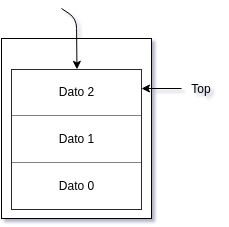
\includegraphics[width=0.3\textwidth]{images/pila}
      
      \end{figure}
    \end{itemize}
        
    
\end{frame}


\subsection{Push}

\begin{frame}
    \frametitle{Push}
    
    \begin{columns}[b]
    \column{0.5\textwidth}
    \begin{figure}
    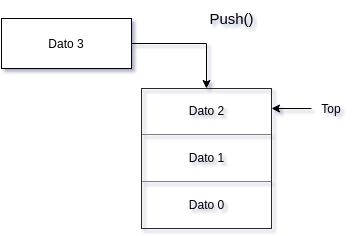
\includegraphics[width =0.9 \textwidth]{images/push1}
    \caption{Inserción de un elemento}
    \end{figure}
   
    \column{0.5\textwidth}
    \begin{figure}
    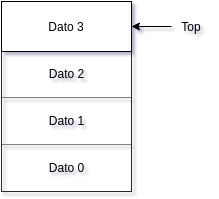
\includegraphics[width =0.65 \textwidth]{images/push2}
    \caption{Pila despues de la inserción}
    \end{figure}
   \end{columns}
    
\end{frame}


\subsection{Pop}
\begin{frame}
    \frametitle{Pop}
    
    \begin{columns}[b]
    \column{0.5\textwidth}
    \begin{figure}
    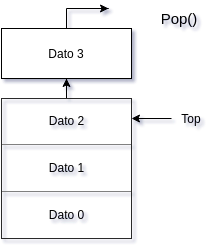
\includegraphics[width =0.8 \textwidth]{images/pop1}
    \caption{Eliminación de un elemento}
    \end{figure}
   
    \column{0.5\textwidth}
    \begin{figure}
    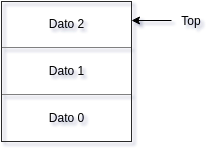
\includegraphics[width =0.8 \textwidth]{images/pop2}
    \caption{Pila despues de eliminar un elemento}
    \end{figure}
   \end{columns}
    
\end{frame}


\subsection{Push - Lista}
\begin{frame}
    \frametitle{Push - Lista}
    
    \begin{figure}
    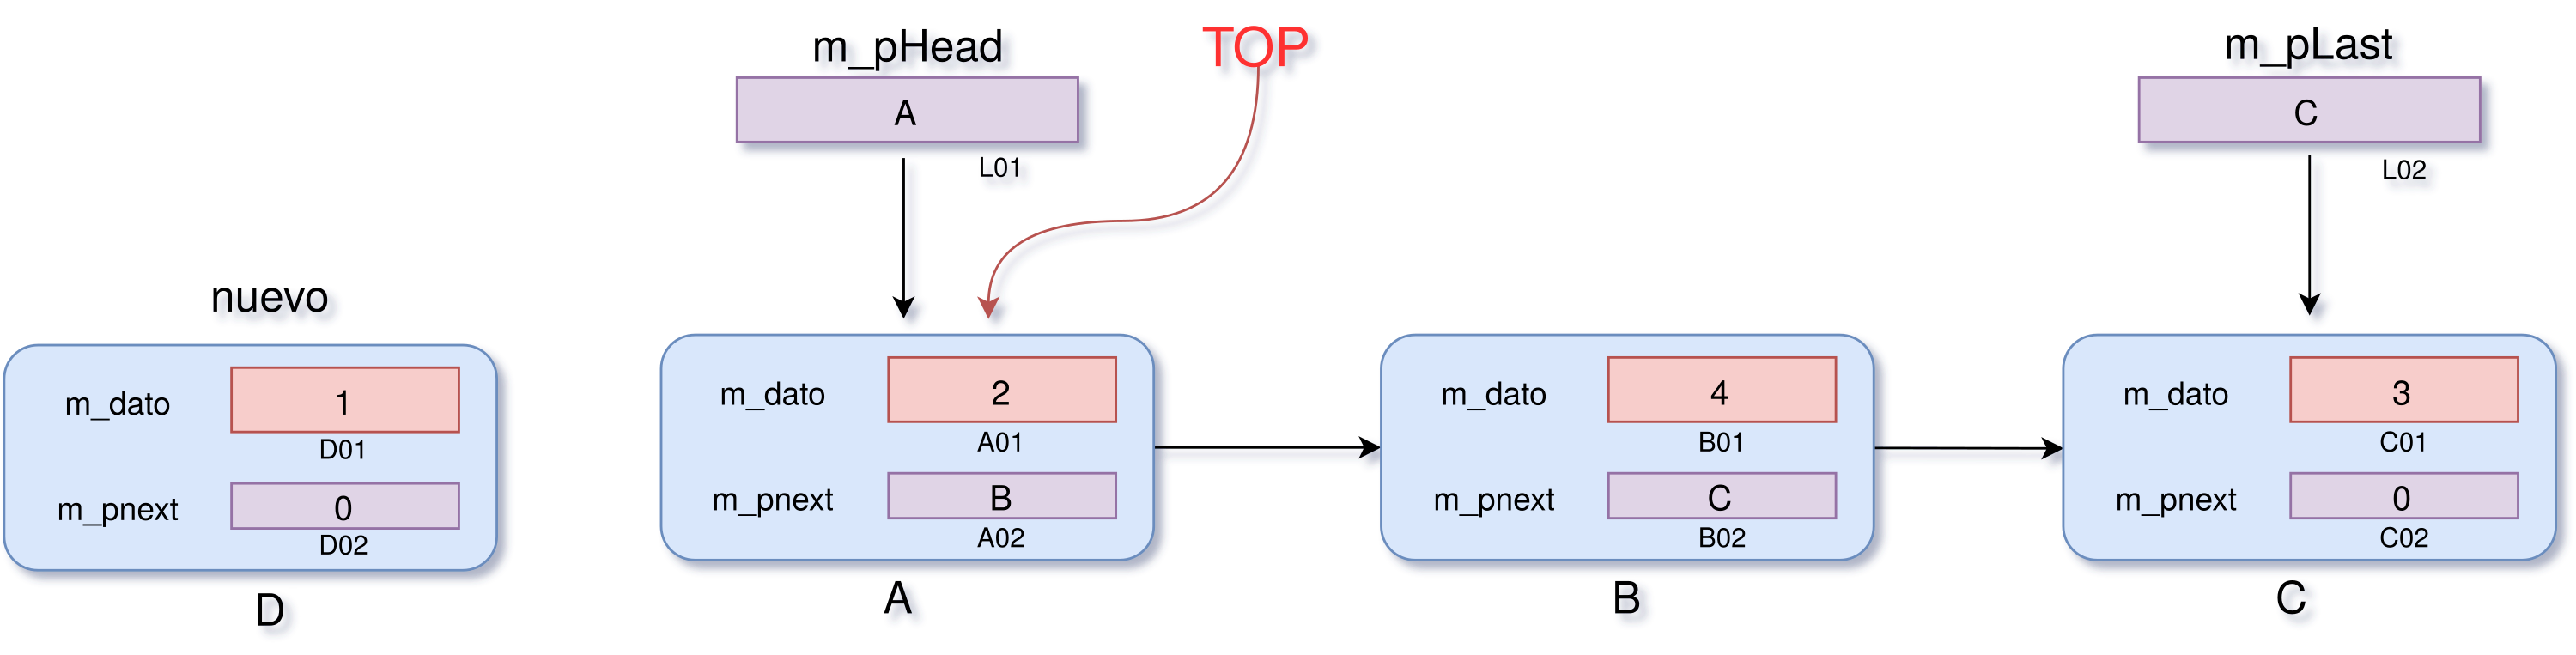
\includegraphics[width =1 \textwidth]{images/push01}
    \caption{Crear nuevo Nodo}
    \end{figure}
       
\end{frame}

\begin{frame}
    \frametitle{Push - Lista}
    
    \begin{figure}
    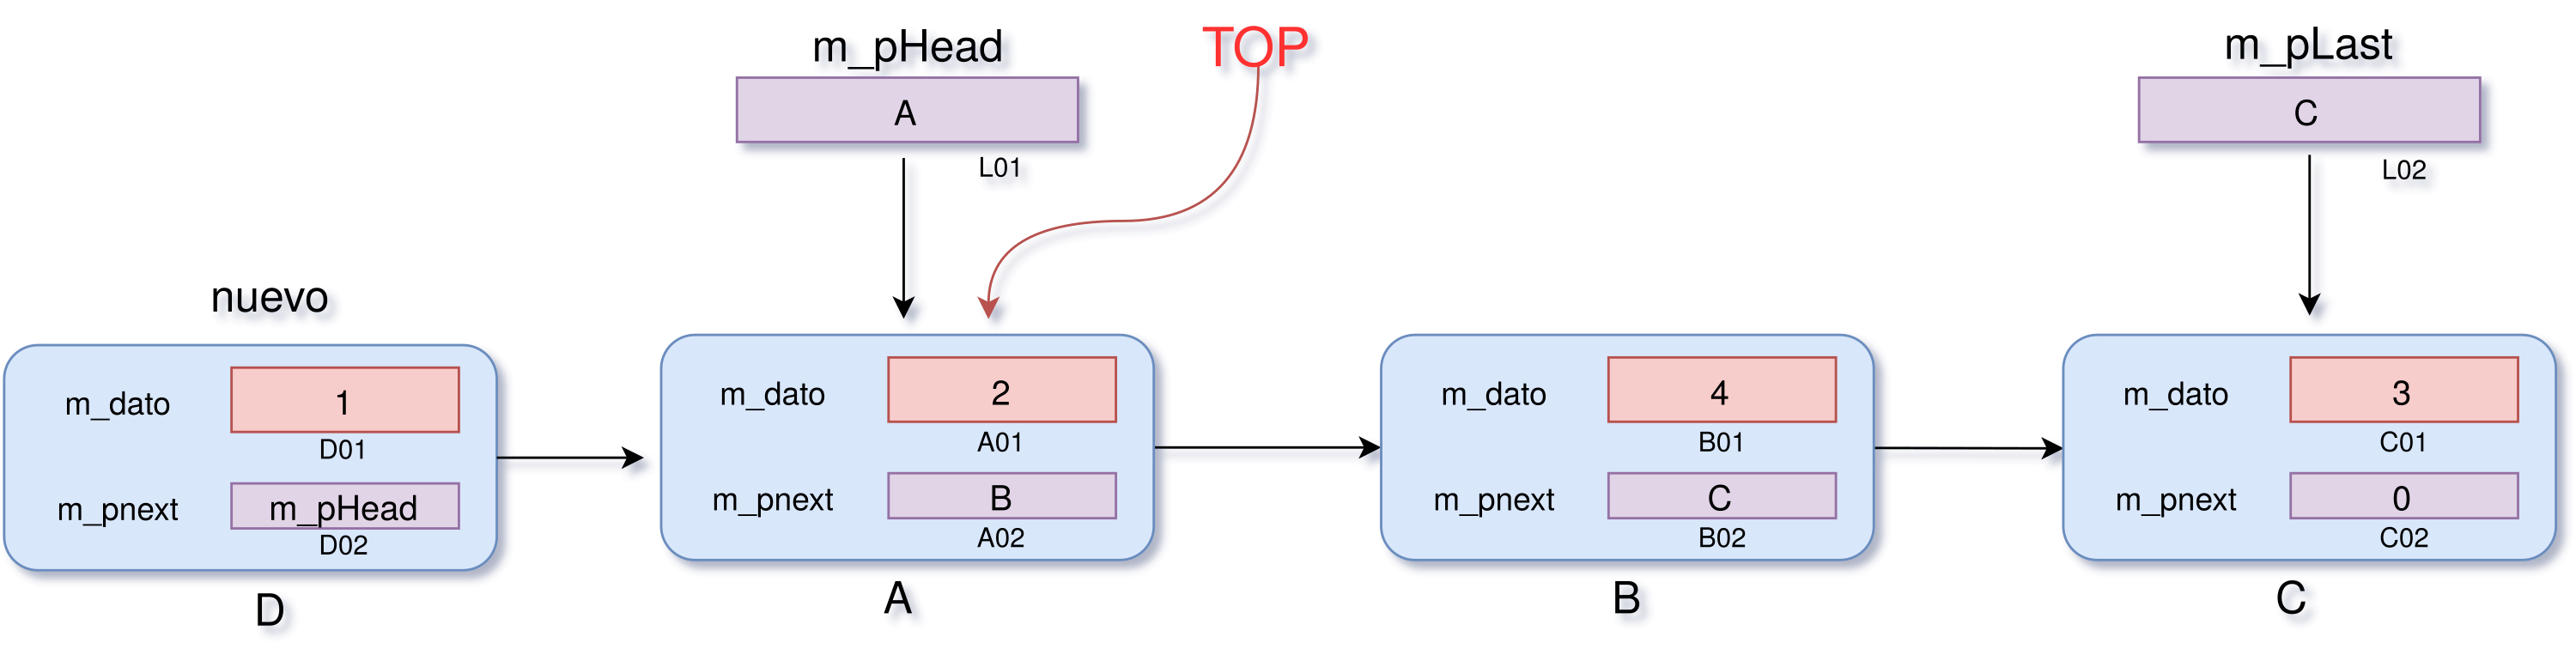
\includegraphics[width =1 \textwidth]{images/push02}
    \caption{Apuntar el Siguiente del Nuevo a la Cabeza de la Lista}
    \end{figure}
       
\end{frame}

\begin{frame}
    \frametitle{Push - Lista}
    
    \begin{figure}
    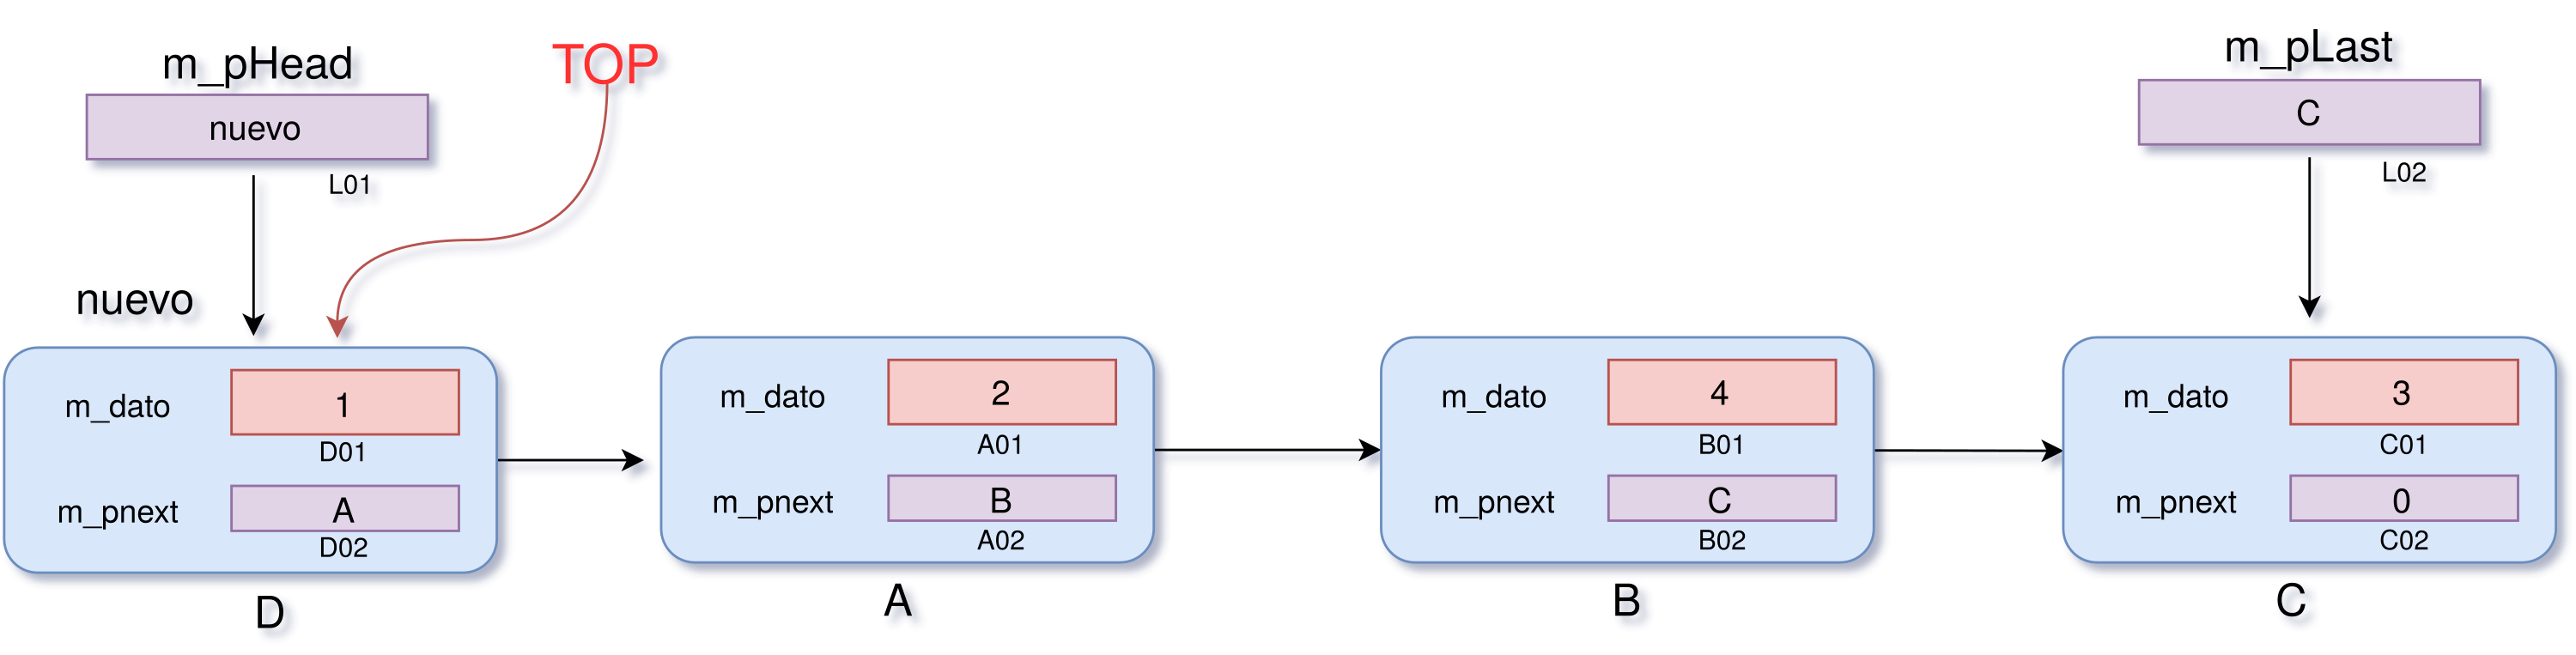
\includegraphics[width =1 \textwidth]{images/push03}
    \caption{Apuntar la Cabeza al Nuevo}
    \end{figure}
       
\end{frame}


\begin{frame}
    \frametitle{Push - Lista}
    
    \begin{figure}
    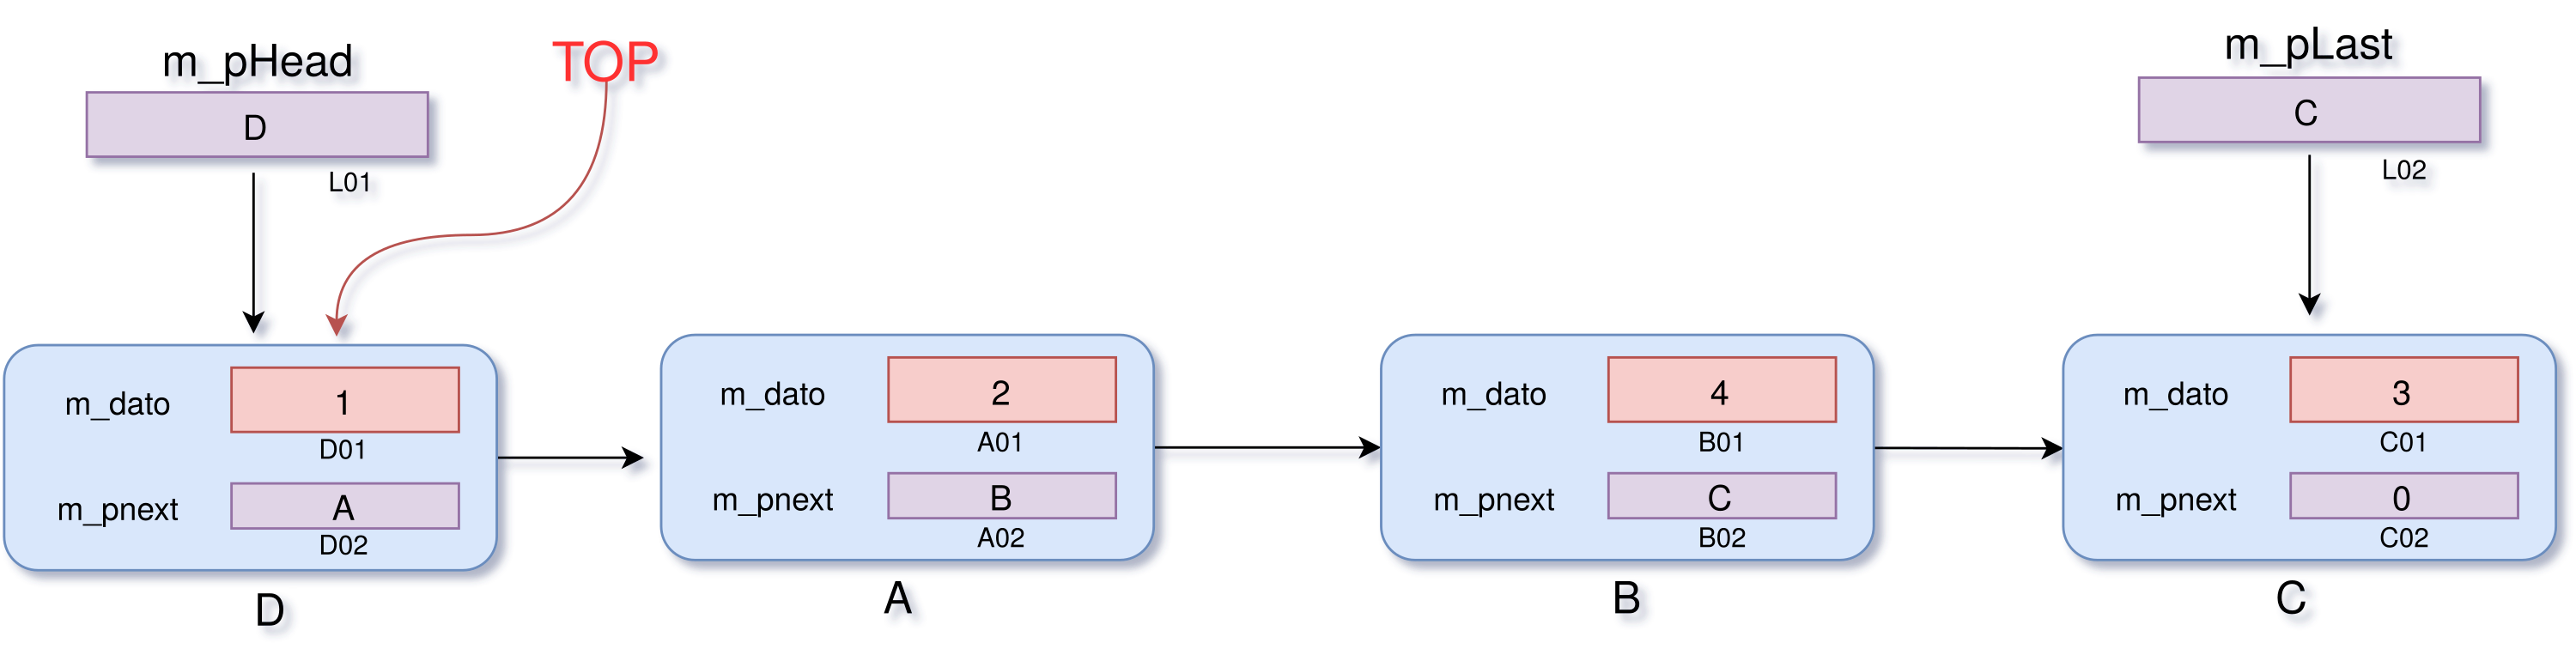
\includegraphics[width =1 \textwidth]{images/push04}
    \caption{Resultado}
    \end{figure}
       
\end{frame}


\subsection{Pop - Lista}
\begin{frame}
    \frametitle{Pop - Lista}
    
    \begin{figure}
    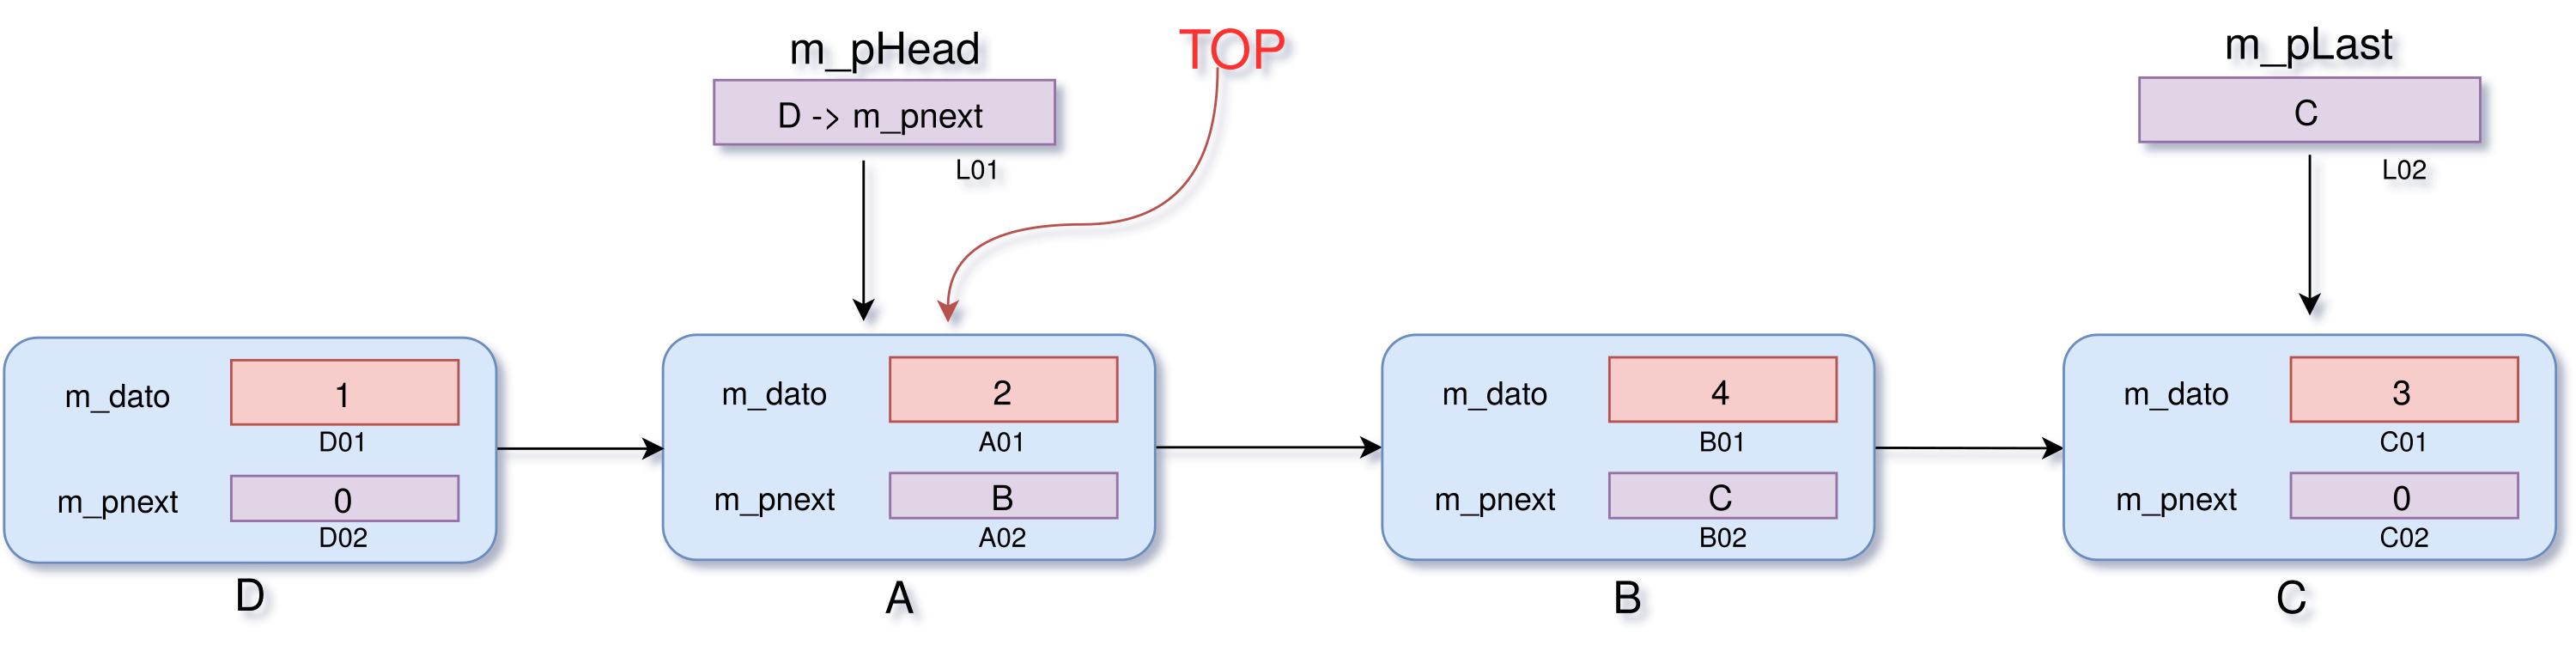
\includegraphics[width =1 \textwidth]{images/pop02}
    \caption{Apuntar la cabeza de la lista al siguiente de la cabeza}
    \end{figure}
       
\end{frame}

\begin{frame}
    \frametitle{Pop - Lista}
    
    \begin{figure}
    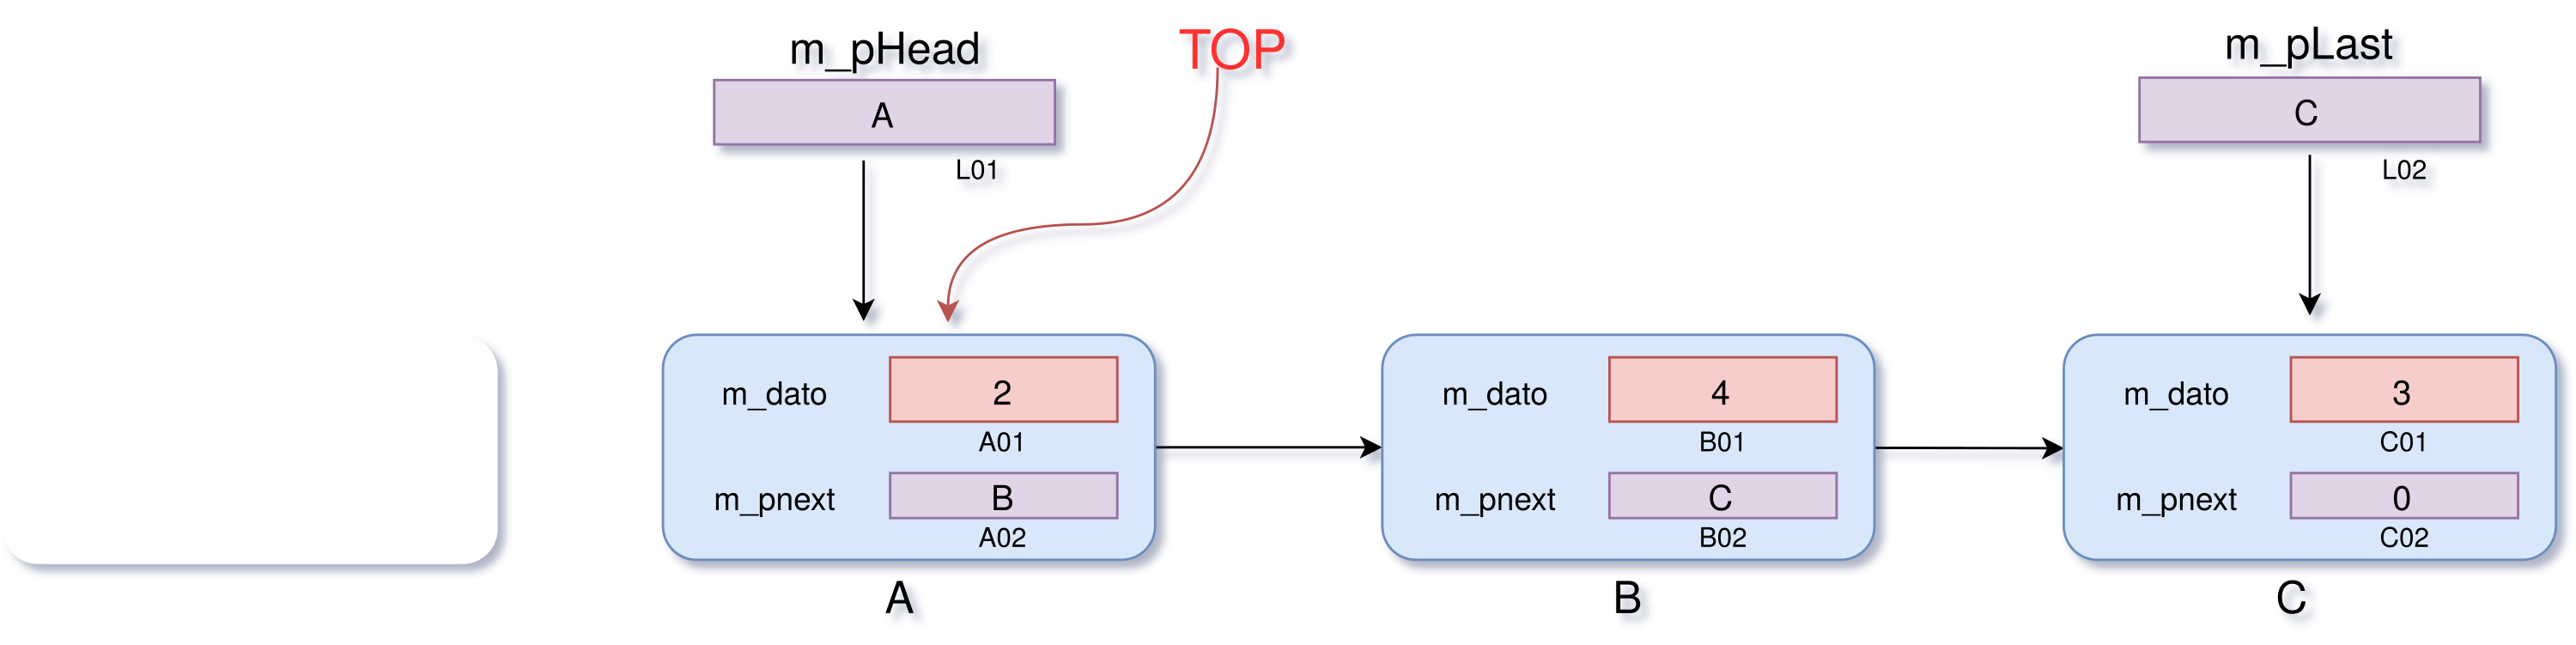
\includegraphics[width =1 \textwidth]{images/pop03}
    \caption{Borrar el nodo y retornar el dato}
    \end{figure}
       
\end{frame}


\section {Colas}
\subsection{Introducción}

\begin{frame}
    \frametitle{Introducción}
    Las colas son caracterizadas por ser una secuencia de elementos en la que la operación de inserción push se realiza por un extremo y la operación de extracción pop por el otro.
    \begin{figure}
    \includegraphics[width =0.7 \textwidth]{imagenes/intro}
    \caption{Una vista rápida}
    \end{figure}
       También se le llama estructura FIFO (del inglés First In First Out).
\end{frame}


%\section{Operaciones}
 \subsection{Encolar-Push}
    \begin{frame}
      \frametitle{Encolar-Push}
      Se añade un elemento al final de esta. Si la cola esta vacía, el elemento es tanto la cabeza como la cola.\\
      .\\
      
      \begin{figure}
    \includegraphics[width =0.3 \textwidth]{imagenes/1push}
    \caption{Insertar caso 1}
    \end{figure}
    \end{frame}
    
    \begin{frame}
	Cuando insertamos un elemento y la cola no esta vacía, este se añade al final de la cola.\\
	Por último actualizamos el último elemento.\\
    
    \begin{figure}
	\includegraphics[width =0.45 \textwidth]{imagenes/2push.png}
      \caption{Insertar caso 2}
      \end{figure}
   
   \end{frame}
    
\subsection{Desencolar-Pop}
    \begin{frame}
      \frametitle{Desencolar-Pop}
      Se elimina el elemento frontal de la cola, el elemento que ingreso primero. 
      .\\
      
      \begin{figure}
	\includegraphics[width =0.7 \textwidth]{imagenes/2pop.png}
      \caption{Eliminar}
      \end{figure}
      
    \end{frame}
    \begin{frame}
      \frametitle{Desencolar-Pop}
      Y actualizamos el primer elemento.
      .\\
      \begin{figure}
	\includegraphics[width =0.5 \textwidth]{imagenes/3pop.png}
	\caption{Actualizar al eliminar}
      \end{figure}
    \end{frame}
    
\subsection{Frente-Front}
    \begin{frame}
      \frametitle{Frente-Front}
      Se devuelve el elemento frontal de la cola, es decir, el primer elemento que entró.\\ 
      .\\
      
      \begin{figure}
	\includegraphics[width =0.7 \textwidth]{imagenes/1frent.png}
     \caption{Devolver elemento frontal}
     \end{figure}
      
    \end{frame}
    \begin{frame}
      \frametitle{Frente-Front}
.
      .\\
      \begin{figure}
	\includegraphics[width =0.2 \textwidth]{imagenes/2frent.png}
    \caption{Resultado}
    \end{figure}
    
    \end{frame}



\section{Bibliografía}
\begin{frame}
\frametitle{Bibliografía}
\begin{thebibliography}{99}

\bibitem{Cd94} Lopez C.[2016].\emph{En Algoritmos y Estructuras de Datos}. Universidad Nacional de San Agustin.

\end{thebibliography}
\end{frame}


\end{document}


